%************************************************
\chapter{Aplicaciones de ZKP}\label{ch:aplicaciones} 
%************************************************


?
Fiat-Shamir para QR, Schnorr para logaritmo discreto, ...
Aplicación de ZKP en los certificados de Idemix. Analizar cómo realizan pruebas de AND, OR, etc.




%TODO: mencionar, para que quede claro en las no interactivas, que los retos pueden no se 0,1


% Hacerlas no interactivas


\section{Firma digital basada en pruebas de conocimiento cero}

Hemos visto que la interacción habitual en una prueba de conocimiento cero es enviar un \textit{testigo}, un \textit{reto} y una \textit{respuesta} en cada iteración.

\begin{center}
	\begin{tabular}{ll}
		P y V & conocen información previa $\Upsilon$
		\\
		P $\rightarrow$ V :& \textit{testigo} $u$
		\\
		V $\rightarrow$ P :& \textit{reto} $b$
		\\
		P $\rightarrow$ V :& \textit{respuesta} $w = \xi(u,b,\Upsilon)$
		\\
		V verifica & $u=\vartheta(b,w,\Upsilon)$.
	\end{tabular}
\end{center}

\hfil

La desventaja de estos protocolos es sincronizar a P y V para comunicarse, por la necesidad de que el verificador debe generar el reto para estar seguro de la prueba (por la propiedad de conocimiento cero).

Una técnica para convertir las pruebas en no interactivas es la \textit{heurística de Fiat-Shamir}, que consiste en sustituir el reto por un resumen digital $h$, \textit{hash} en inglés, del testigo $u$, de modo que para un P computacionalmente limitado, V puede confiar en que P no ha elegido $u$ tal que con el reto calculado pueda falsear la prueba.

Aprovechando la función del \textit{hash}, se puede convertir el protocolo en un esquema de firma digital de un mensaje $m$, realizando el \textit{hash} sobre el testigo y el mensaje a la vez (concatenándolos, por ejemplo).


\begin{center}
	\begin{tabular}{ll}\label{fiat-shamir-heur}
		P calcula :& \textit{testigo} $u$, \textit{respuesta} $w = \xi(u, h,\Upsilon)$, donde $h=$\textbf{hash(u|m)}
		\\
		P $\rightarrow$ V :& \textit{\textbf{firma del mensaje}} $m$: \quad $(h,w)$
		\\
		V verifica & $h=hash(\vartheta(h,w,\Upsilon)|m)$.
	\end{tabular}
\end{center}

Podemos construir así una firma digital, con un solo mensaje, por lo que es válido para cualquier V, y donde P no ha debido compartir ninguna clave o información extra aparte de los parámetros del sistema, $\Upsilon$.

\hfil


\begin{remark}
	\hfil
	
	En las pruebas de conocimiento cero perfectas estudiadas, los retos consistían en un bit, por lo que los posibles valores son $0$ ó $1$ y un ataque a la función de \textit{hash} es muy fácil. Por ello, se utilizan versiones de ZKP donde el conjunto de los posibles valores del reto es suficientemente grande, por ejemplo, un entero representado en tantos bits como produce la firma digital, usualmente 256 o 512 bits.
	
	Al hacer este cambio, muchas veces perdemos la condición de perfecta en la prueba de conocimiento cero, rebajándola a otro de los tipos vistos, pero que en la práctica es perfectamente aceptable.
	
\end{remark}








\section{Protocolos de identificación basados en ZKP}
% Fiat-Shamir, FFS, GQ, Schnorr


Las pruebas de conocimiento cero tienen una gran aplicación en el campo de la seguridad informática, en particular en la \textbf{autenticación}. Tras la autenticación se aplicará autorización y control de acceso, por eso es importante un sistema de identificación fiable. Además, de entre las ventajas de las pruebas de conocimiento cero, un sistema de identificación basado en ZKP hereda privacidad, al no revelar información del usuario, y seguridad al no \textit{degradarse} con el uso, es decir, resiste al criptoanálisis por muchos mensajes que se intercepten, y ataques con mensajes elegidos. 

%TODO
TODO: redactar mejor las ventajas.

Estos protocolos de identificación se basan en una prueba de conocimiento cero de un problema $Q$, donde P (el usuario) tiene un \textit{secreto} que le permite demostrar una instancia $Verdadera$ de $Q$ al verificador V, y que además conocer dicho secreto le relaciona con una identidad, con la ventaja de no tener que revelar el secreto.


\subsection{Protocolo de identificación de Fiat-Shamir}

El protocolo  de identificación más característico basado en ZKP y el problema QR es el de Fiat-Shamir.

Como hemos visto, el problema QR es \textbf{NP}, de modo que obtener una raíz cuadrada módulo un $N$ compuesto, es computacionalmente inviable, equivalente a factorizar $N$. Bajo esta suposición, podemos utilizar como información pública un residuo cuadrático módulo $N$, que llamaremos $v$, y asociarlo a una identidad, de modo que el usuario que conozca una de sus raíces cuadradas, el secreto $s$, podrá demostrar que $v$ es un residuo cuadrático por medio de una prueba de conocimiento cero.


\rule{\textwidth}{1pt}
\begin{algorithm}[Protocolo de identificación Fiat-Shamir]
	\hfil
	
	\textit{Configuración de la identidad}:
	\begin{enumerate}
		\item La entidad de confianza selecciona y publica $N=pq$, con $p$ y $q$ primos y secretos.
		
		\item Cada usuario P genera un secreto $s \in \mathbb{Z_N^*}$, coprimo con $N$ (si no, se podría obtener la factorización de $N$ y perder la seguridad del protocolo). Calcula $v \equiv s^2 \, mod \, N$ y lo envía a la entidad de confianza como su clave pública.
		
	\end{enumerate}
	
	
	\textit{Protocolo}: Repetir $t$ rondas:
	\begin{enumerate}
		\item P escoge aleatoriamente $r \in_R \mathbb{Z_N^*}$, el \textit{compromiso}.
		\item $P \rightarrow V$:\quad $u \equiv r^2 \, mod \, N$, el \textit{testigo}.
		\item $V \rightarrow P$:\quad $b \in_R \{0,1\}$, el \textit{reto}.
		\item $P \rightarrow V$:\quad $w \equiv r\cdot s^b \, mod \, N$, la \textit{respuesta}.
		\item V verifica si \quad $ w^2 \equiv u\cdot v^b \, mod \, N$.
	\end{enumerate}
	
\end{algorithm}
\rule{\textwidth}{1pt}

\hfil


El protocolo de Fiat-Shamir es casi idéntico a la prueba interactiva \ref{QRinteractive:alg}, donde aquí $(v,N)$ hace el papel de instancia $Verdadera$ del problema QR, y como P, el usuario, es una máquina computacionalmente limitada, en vez de elegir aleatoriamente el residuo cuadrático $u$ y la raíz cuadrada $w$, parte de las raíces cuadradas, $s$ y $r$, para poder calcular $u$, $v$ y $w$ elevando al cuadrado. Como los valores que se envían siguen siendo $u$, un residuo cuadrático aleatorio, $b$ un bit de reto, y $w$ una raíz cuadrada aleatoria de $u$ o $uv$, según $b$, las transcripciones del protocolo de Fiat-Shamir son las mismas que las de la prueba interactiva, que sabemos que es de conocimiento cero perfecta.

\hfil

El intento de ataque que vimos en la demostración de robustez varía ligeramente para Fiat-Shamir, pues el objetivo es intentar demostrar que $v$ es residuo cuadrático, sin conocer $s$ u otra raíz cuadrada, necesaria para una máquina de cómputo limitado del mundo real.

Un atacante debe adivinar el bit del reto que recibirá, de modo que si cree que $b=0$ calcula el testigo como en el protocolo, pero si cree que $b=1$, calcula en el paso 2 el testigo $u \equiv r^2\cdot v^{-1} \, mod \, N$, y en 4 la respuesta $w \equiv r \, mod \, N$. En ambos casos fallaría si no adivina $b$ correctamente, pues para corregir su error debería ser capaz de calcular, respectivamente, una raíz cuadrada de $v$, que permitiría pasar la prueba siempre, o una raíz cuadrada de $u \equiv r^2\cdot v^{-1} \, mod \, N$, computacionalmente inviable pues $p$ y $q$ los guarda como secretos la entidad de verificación.

Como en la prueba interactiva, un atacante tiene una probabilidad de $1/2$ de engañar a V en cada ronda, de modo que la robustez se mantiene con una probabilidad de ataque de $2^{-t}$. Si P pasa correctamente las $t$ rondas, V da por válida la prueba. Si falla aunque sea sólo una, rechaza la identificación.

\hfil

Un detalle importante a tener en cuenta es que, considerando ordenadores reales para el caso práctico, si P no utiliza un buen generador de números aleatorios para sus $r$ del paso 1, un atacante podría adivinar cuándo repetirá el $r$, mandar $b=0$ y $b=1$, y así calcular el secreto $s$.




\subsection{Protocolo de identificación de Feige-Fiat-Shamir}

% TODO: no estoy convencido de poner este. En el Fiat-Shamir el protocolo es prácticamente la prueba de conocimiento cero formal, aquí se intuye que se basa en la dificultad de QR, pero ya está.

Una variación del protocolo de Fiat-Shamir para disminuir el número de mensajes intercambiados combinando varios testigos y retos a la vez.

\rule{\textwidth}{1pt}
\begin{algorithm}[Protocolo de identificación Feige-Fiat-Shamir]
	\hfil
	
	\textit{Configuración de la identidad}:
	\begin{enumerate}
		\item \textit{Parámetros del sistema}: La entidad de confianza publica el módulo $N=pq$, con $p$ y $q$ $\equiv \, mod \, 4$, primos guardados secretos, de modo que $-1$ es un no-residuo cuadrático con símbolo de Jacobi 1. También define los enteros $k$ y $t$ que definen la seguridad.
		
		\item \textit{Selección del secreto}: Cada usuario P hace:
		
		\subitem (a) Selecciona aleatoriamente un vector $(s_1,s_2,\dots ,s_k)$, donde cada  $s_i \in \mathbb{Z_N^*}$ y $mcd(s_i, N)=1$. Además, elige también aleatoriamente $k$ bits $(b_1, b_2, \dots , b_k)$.
		
		\subitem (b) Calcula $v_i \equiv (-1)^{b_i}\cdot (s_i^2)^{-1} \, mod \, N$ para cada $i=1,\dots k$.
		
		\subitem (c) El usuario se identifica ante la entidad de confianza y envía su \textit{clave pública} $(v_1,\dots , v_k; N)$, y guarda su \textit{clave privada} $(s_1, \dots , s_k)$.
		
	\end{enumerate}
	
	
	\textit{Protocolo}: Repetir $t$ rondas:
	\begin{enumerate}
		\item P escoge aleatoriamente $r \in_R \mathbb{Z_N^*}$ y un bit $b \in_R \{0,1\}$.
		\item $P \rightarrow V$:\quad $u \equiv (-1)^b \cdot r^2 \, mod \, N$, el \textit{testigo}.
		\item $V \rightarrow P$:\quad $(b_1,\dots ,b_k)$, con cada $b_i \in_R \{0,1\}$, el \textit{reto}.
		\item $P \rightarrow V$:\quad $w \equiv r\cdot \prod_{j=1}^{k} s_j^{b_j} \, mod \, N$, la \textit{respuesta}.
		\item V verifica si \quad $ u \equiv \pm \, w^2 \cdot \prod_{j=1}^{k} v_j^{b_i} \, mod \, N$.
	\end{enumerate}
	
\end{algorithm}
\rule{\textwidth}{1pt}

La probabilidad de que un atacante pueda engañar a V es la de acertar el reto de $k$ bits en cada una de las $t$ rondas, es decir, $2^{-kt}$. Como vemos, aumentando el número de retos por ronda, podemos reducir el número de mensajes intercambiados para conseguir una robustez equivalente a Fiat-Shamir.



%TODO GQ
% TODO:
% Si en los preliminares de QR ampliamos a la dificultad de solucionar una raíz n-ésima, podemos meter Guillou-Quisquater (GQ), y dejar caer que es ZKP al ser una extensión de Fiat-Shamir, o demostrar formalmente que es ZKP (~).


\subsection{Protocolo de identificación de Schnorr}

% https://crypto.stackexchange.com/questions/9997/perfect-zero-knowledge-for-the-schnorr-protocol

% Indican que demostrar que Schnorr es ZKP con un challenge grande no se puede, porque no se conoce un simulador eficiente

Este protocolo se basa en el problema del logaritmo discreto


\rule{\textwidth}{1pt}
\begin{algorithm}[Protocolo de identificación Schnorr]
	\hfil
	
	\textit{Configuración de la identidad}:
	\begin{enumerate}
		\item \textit{Parámetros del sistema}: La entidad de confianza publica los parámetros $(p,q,\beta)$ donde $p$ y $q$ son primos tal que $q\mid (p-1)$, y $\beta$ es un elemento con orden multiplicativo $q$ (por ejemplo, para $\alpha$ un generador $mod\,p$, $\beta=\alpha^{(p-1)/q}\,\mod\,p$). Además se escoge un $t$, $2^t < q$, que definirá el nivel de seguridad.
		
				
		\item \textit{Selección del secreto}: Cada usuario P:
		
		\subitem (a) Recibe una identidad única $I_P$.
		
		\subitem (b) Escoge una clave privada $a$, $0\leq a \leq q-1$, y calcula $v = \beta^{-a}\, mod\, p$.
		
		\subitem (c) La entidad certificadora vincula la identidad $I_P$ y el valor $v$ firmando, con cualquier método de firma $S()$, el certificado $cert_A = (I_P, v, S_T(I_P|v))$.
		
	\end{enumerate}
	
	
	\textit{Protocolo}:
	\begin{enumerate}
		\item P escoge aleatoriamente $r$, $0\leq r\leq q-1$, y un calcula $x=\beta^r\,mod\,p$.
		\item $P \rightarrow V$:\quad $x$, el \textit{testigo}, y $cert_P$.
		\item $V \rightarrow P$:\quad $e$ aleatorio, $1\leq e\leq 2^t<q$, el \textit{reto}, y verifica la firma del certificado.
		\item $P \rightarrow V$:\quad $y=ae+r\, mod\, q$, la \textit{respuesta}.
		\item V verifica si \quad $ x = \beta^y v^e \, mod \, p$.
	\end{enumerate}
	
\end{algorithm}
\rule{\textwidth}{1pt}

\hfil

Un P malicioso tiene una probabilidad de $2^-t$ de adivinar el reto, pero esta prueba no es una prueba de conocimiento cero perfecta, pues como vimos en el capítulo anterior, el simulador en tiempo polinomial existe si los retos $e$ tienen un dominio pequeño. Como se menciona en \citep{idemixSpec}, esta prueba es de conocimiento cero con verificador honesto (el que sigue el protocolo eligiendo el reto aleatoriamente), pero eligiendo un reto en un espacio de valores menor logarítmico respecto el parámetro $t$, y realizando múltiples iteraciones, se puede conseguir la condición de \textit{perfecta}, a cambio de perder eficiencia. También se indica que de \citep{Dam00} se pueden tomar construcciones para transformarlo en una prueba de conocimiento cero manteniendo eficiencia.


% TODO : ejemplo


\subsubsection{Probar el conocimiento de una representación}\label{reprKP}

Una generalización de Schnorr es utilizar $l$ bases $g_1, \dots, g_l$ con $g_i \in G = <g>$, un grupo de orden $o(g)=q$ primo. Sea $y\in G$ tal que conocemos los valores $x_1,\dots,x_l$ que cumplen $y = \prod_{i=1}^{k} g_i^{x_i}$. Una prueba de conocimiento cero de que conocemos la representación de $y$ con respecto a las bases $g_1, \dots, g_l$ es:


\rule{\textwidth}{1pt}
\begin{algorithm}
	P y V conocen $y$, $g_1, \dots, g_l$, $q$ y el parámetro del sistema $k$.
	
	\hfil
	
	Repetir $t$ rondas:
	\begin{enumerate}
		\item P escoge aleatoriamente $l$ enteros $r_i \in_R \mathbb{Z_q}$.
		\item $P \rightarrow V$:\quad $t=\prod_{i=1}^{l}g_i^{r_i}$.
		\item $V \rightarrow P$:\quad $c \in_R \{0,1\}^k$, un entero aleatorio de $k$ bits.
		\item $P \rightarrow V$:\quad $s_i = r_i - c\cdot x_i \, mod \, q$, para $i=1,\dots,l$.
		\item V verifica si \quad $t = y^c \prod_{i=1}^{l} g_i^{s_i}$.
	\end{enumerate}
	
\end{algorithm}
\rule{\textwidth}{1pt}

La probabilidad de que un P malicioso adivine los $k$ bits aleatorios del reto $c$ es de $2^{-k}$. Este tipo de prueba se utiliza en Idemix, del cual hablaremos en la siguiente sección.


%
%
%
%
%





\section{Pruebas de conocimiento cero en Identity Mixer}

Identity Mixer, o Idemix, es un protocolo desarrollado por IBM\footnote{Identity Mixer - \url{https://www.research.ibm.com/labs/zurich/idemix/}} para crear certificados digitales basados en atributos, donde se preserva la privacidad. Este protocolo no solo permite la autenticación sin revelar un valor secreto, también permite realizar pruebas sobre los atributos del certificado de un usuario, sin revelar los valores, como por ejemplo, ``\texttt{año\_actual - año\_nacimiento $\geq$ 18}''.

Los protocolos criptográficos en los que se especifican en Idemix \citep{idemixSpec} han sido desarrollados durante años por expertos en el área, donde destacan Jan Camenisch y Anna Lysyanskaya con el desarrollo de la firma CL \citep{camenisch2002signature} \citep{camenisch2001efficient} que se utiliza para firmar certificados sin tener que conocer los valores de todos los atributos, y que permite posteriormente al usuario demostrar que posee dicha firma, sin desvelarla. Esto permite poder utilizar múltiples veces un certificado de manera anónima sin que se relacionen los diferentes usos con la misma persona.





\subsection{Notación para ZKP}

Como hemos visto, cualquier problema de decisión posee una prueba de conocimiento cero, y de entre esas pruebas, las pruebas de conocimiento de un secreto son las que se utilizan en los certificados. Utilizaremos la siguiente notación de Camenisch y Stadler \citep{camenisch1997efficient} para denotar una prueba de conocimiento cero de conocimiento de un secreto.

\begin{center}
	$ZKPoK\{ (w) : \mathcal{L}(w,x) \}$
\end{center}
donde $w$ es un testigo, normalmente el secreto, $x$ es información conocida por ambas partes, y $\mathcal{L}(w,x)$ es un predicado que representa una condición sobre $w$ y $x$. Se puede leer como ``conozco un testigo $w$ tal que el predicado $\mathcal{L}(w,x)$ se cumple para $w$ y $x$''. Para abreviar, en vez de ZKPoK (\textit{Zero-Knowledge Proof of Knowledge}), usaremos ZKP o PK.

\hfil

Por ejemplo,
\begin{center}
	$PK\{ (\alpha) : y=g^\alpha \}$
\end{center}
donde $y\in G = <g>$, un grupo de orden $q$ primo, denota el protocolo de identificación de Schnorr.


\subsection{Combinar diferentes pruebas de conocimiento}

Cuando leamos pruebas de conocimiento con varias condiciones, como
\begin{center}
	$$
	PK\{ (\alpha_1,\dots,\alpha_l,\beta_1,\dots,\beta_{l`}) : y=\prod_{i=1}^{l}g_i^{\alpha_i} \wedge z=\prod_{i=1}^{l`}h_i^{\beta_i} \}
	$$
\end{center}
con $g_i,h_i,y,z\in G$, será equivalente a realizar de manera paralela e independiente cada protocolo:
\begin{center}
	$$
	PK\{ (\alpha_1,\dots,\alpha_l) : y=\prod_{i=1}^{l}g_i^{\alpha_i} \}
	$$
	y
	$$
	PK\{ (\beta_1,\dots,\beta_{l`}) : z=\prod_{i=1}^{l`}h_i^{\beta_i} \}
	$$
\end{center}


En el primer mensaje, P envía los testigos de cada uno de los protocolos. Entonces, V envía un único reto, el mismo para cada protocolo. Finalmente, P responde al reto con la respuesta de cada prueba, y V las verifica.



\subsection{Firma Camenisch-Lysyanskaya}

El esquema de firma de Camenisch-Lysyanskaya, o firma CL, es la base de los certificados Idemix. 

Sean $p`$ y $q`$ dos primos, tal que $p=2p`+1$ y $q=2q`+1$ también lo son, llamados \textit{primos seguros}. Los parámetros del sistema, conocidos por el firmante y quien comprueba la firma son: el entero $n=pq$, $Z,S,R\in QR_n$ (grupo multiplicativo de los residuos cuadráticos módulo $n$). La clave secreta del firmante es $(p,q)$ y el mensaje lo denominaremos $m$. La firma CL sobre $m$ es la tupla $(A,e,v)$ tal que
\begin{center}
	$A \equiv \left( \dfrac{Z}{S^v R^m} \right) ^{1/e} \, mod \, n$
\end{center}
donde $e,v$ son aleatorios, $e$ primo y $\frac{1}{e}\cdot e \equiv 1 \, mod \, \varphi(n)$.


Para comprobar que una firma $(A,e,v)$ es correcta, basta comprobar si
\begin{center}
	$Z \overset{?}{\equiv} A^e S^v R^m \, mod \, n$.
\end{center}

\hfil

La ventaja de esta firma es que se puede aplicar sobre múltiples mensajes a la vez, que en el caso de un certificado, serán los diferentes atributos a firmar. En este caso los parámetros del sistema se mantienen, $n=pq$, $Z,S\in QR_n$, pero debemos calcular un residuo cuadrático por cada mensaje a firmar, $R_0,\dots,R_l\in QR_n$. La clave secreta sigue siendo $(p,q)$, y la firma de los mensajes $m_0,m_1,\dots,m_l$ es $(A,e,v)$ tal que
\begin{center}
	$A \equiv \left( \dfrac{Z}{S^v \prod_{i=0}^{l} R_i^{m_i} } \right) ^{1/e} \, mod \, n$
\end{center}

\hfil

Para verificar la firma, comprobamos que
\begin{center}
	$Z \overset{?}{\equiv} A^e S^v \prod_{i=0}^{l} R_i^{m_i} \, mod \, n$.
\end{center}


La firma CL se basa en la \textit{suposición RSA fuerte}, donde tanto el problema RSA y el del logaritmo discreto son difíciles de resolver a la vez, es decir, dado un módulo RSA $n$, y un valor $u\in \mathbb{Z}_n^*$, es difícil calcular una pareja de valores $(e,v)$, tal que $v^e \equiv u \, mod \, n$.



Como el firmante conoce los factores primos $p$ y $q$ de $n$, puede calcular, utilizando el Teorema Chino de los Restos, la firma fácilmente, pero quien no la conoce, se enfrenta al problema anterior para deshacer los cálculos.


\subsection{Firma Camenisch-Lysyanskaya aleatorizada}\label{CLrandomized}

Dada una firma CL $(A,e,v)$, sobre los mensajes  $m_0,m_1,\dots,m_l$, podemos obtener una firma $(\acute{A},e,\hat{v})$ distinta de la anterior, excepto por $e$, y todavía válida. Esta nueva firma la puede generar cualquier usuario, pues no precisa del secreto $(p,q)$ de la firma original.

La nueva firma se calcula a partir de un entero aleatorio $r$, tal que $\acute{A}= A\cdot S^{-r}\, mod\, n$ y $\hat{v}=v+er$.

La verificación de $(\acute{A},e,\hat{v})$ se realiza igual que en la original, ya que:

\begin{center}
	$
	\acute{A}^e S^{\hat{v}} \prod_{i=0}^{l} R_i^{m_i} \equiv A^e S^{-er} S^v S^{er} \prod_{i=0}^{l} R_i^{m_i} \equiv A^e S^v \prod_{i=0}^{l} R_i^{m_i} \equiv Z \, mod \, n
	$
\end{center}


\subsection{Firma de credenciales Idemix}

En la expedición del certificado intervienen el Usuario y el Emisor (por ej., una compañía o gobierno). Durante el protocolo de emisión, el Usuario y el Emisor calculan interactivamente una firma CL, es decir, entre los dos generarán la firma CL, porque ninguno tendrá toda la información necesaria para generar la firma por sí mismo. En cada paso, una prueba de conocimiento cero asegurará que cada parte ha seguido el protocolo.

El Emisor conocerá la factorización de $n$, mientras que el Usuario guardará su clave secreta, $m_0$ y, opcionalmente, los atributos del certificado, $m_1,\dots,m_l$. Al final de la firma, el Usuario conocerá una representación, $(m_1,\dots,m_l)$ de $\frac{Z}{A^eS^v}$ con respecto a la base $(R_0,\dots,R_l)$, y como ya hemos visto, podrá demostrar con una prueba de conocimiento cero que conoce dicha representación sin revelar ninguno, o solo un subconjunto. Además, el Emisor no conocerá la firma $(A,e,v)$ final, pues $v$ se calculará también de manera conjunta de modo que sólo el Usuario conocerá el valor final.

\hfil

A continuación presentamos una versión simplificada del protocolo, donde los atributos son conocidos por el Emisor. En otras versiones el Usuario puede enviar pruebas sobre alguna propiedad del atributo, o pseudónimos, sin revelar el verdadero valor al Emisor. Es importante notar que el número de residuos cuadráticos generados por el emisor, $R_0,\dots,R_{l'}$ determina el máximo de atributos que puede llevar un certificado.

\rule{\textwidth}{1pt}
\begin{algorithm}[Emisión de certificado Idemix]
	\hfil
	
	\textit{Conocimiento común}: $n,Z,S,R_0,\dots,R_{l'},m_1,\dots,m_l$, donde $l'\geq l$
	
	\textit{Conocimiento del Emisor}: $p,q$ tal que $n=pq$.
	
	\textit{Conocimiento del Usuario}: $m_0$, su clave secreta.
	
	\hfil
	
	\textit{Protocolo}:
	\begin{enumerate}
		\item Ronda 1: Emisor
		\begin{enumerate}[label*=\arabic*.]
			\item El Emisor escoge un valor aleatorio $n_1$ y lo envía al Usuario.
		\end{enumerate}
		
		\item Ronda 2: Usuario
		\begin{enumerate}[label*=\arabic*.]
		
			\item El Usuario elige un valor $v'$ aleatorio (primer paso para calcular el $v$ de la firma).
			
			\item Calcula el valor $U = S^{v'} \cdot R_0^{m_0} \, mod \, n$.
			
			\item Calcula* la prueba $P_1 := ZKP\{(\nu',\mu_0) : U \equiv S^{\nu'}R_0^{\mu_0} \, mod \, n \}(n_1)$, no interactiva, dependiente de $n_1$.
			
			\item Envía $U,P_1,n_2$, donde $n_2$ es un valor aleatorio elegido por el Usuario.

		\end{enumerate}

		\item Ronda 3: Emisor firma CL
		\begin{enumerate}[label*=\arabic*.]
			\item Verifica* la prueba $P_1$ del Usuario.
			
			\item Elige un valor un $e$ primo y $v''$ aleatorios (segundo paso para calcular el $v$ de la firma).
			
			\item Calcula el valor $A = \left(  \dfrac{Z}{U\cdot S^{v''}\cdot \prod_{i=1}^{l} R_i^{m_i}} \right)^{1/e} \, mod \, n$.
			
			\item Calcula* $P_2 := ZKP\{(\delta) : A \equiv \left( \dfrac{Z}{U\cdot S^{v''}\cdot \prod_{i=1}^{l} R_i^{m_i}} \right)^{\delta} \, mod \, n \}(n_2)$, no interactiva, dependiente de $n_2$.
			
			\item Envía $(A,e,v'')$ y $P_2$ al Usuario.
		\end{enumerate}
		
		
		\item Ronda 4: Usuario
		\begin{enumerate}[label*=\arabic*.]
			\item Calcula $v=v'+v''$.
			\item Verifica $P_2$ y la firma CL $(A,e,v)$.
		\end{enumerate}

	\end{enumerate}
	
\end{algorithm}
\rule{\textwidth}{1pt}



\begin{flushleft}
	*A continuación mostramos las pruebas y verificaciones correspondientes.
\end{flushleft}

\begin{figure}[bth]
	\begin{center}
		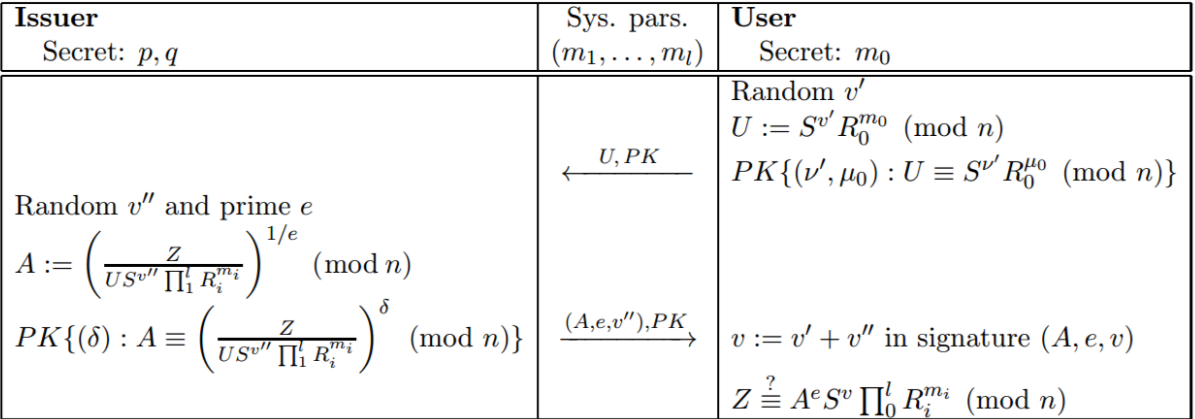
\includegraphics[width=\linewidth]{gfx/issuanceIdemix}
	\end{center}
	\caption{Idemix: firma de credenciales simplificada.}
	\label{fig:issuanceIdemix}
\end{figure}

\hfil


La prueba de conocimiento $P_1$ indica que conocemos un $v'$, primera parte del $v$ final de la firma CL, y un $m_0$, nuestra clave secreta, tales que $U$ se representa como $(v', m_0)$ en la \textit{base} $(S,R_0)$. Utilizando la heurística de Fiat-Shamir, en vez de pedir varios retos al Emisor para conseguir robustez, utilizamos una función de hash junto a un reto $n_1$ del emisor, llamado en inglés \textit{nonce}. La prueba que se envía consiste en el reto obtenido con el hash, y las respuestas a dicho reto.

\begin{algorithm}[$KP\{(v',m_0) : U \equiv S^{v'}R_0^{m_0} \, mod \, n \}(n_1)$]
	\hfil
	
	\begin{enumerate}
		\item Elegir $\tilde{m}_0$ y $\tilde{v}'$ aleatorios.
		\item Calcular $\tilde{U} = S^{\tilde{v}'}\cdot R_0^{\tilde{m}_0} \, mod \, n$.
		\item Reto por heurística Fiat-Shamir: $c = H(U||\tilde{U}||n_1)$.
		\item Respuestas al \textit{reto}: $\hat{v}' = \tilde{v}' + c v'$, $\hat{m}_0 = \tilde{m}_0 + c m_0$.
		\item $P_1 := (c, \hat{v}', \hat{m}_0)$.
	\end{enumerate}
	
\end{algorithm}

\hfil

Para verificar la prueba anterior, por la heurística de Fiat-Shamir (\ref{fiat-shamir-heur}), debemos \textit{recuperar} el valor de $U$ calculado por el Usuario, y comparar los hashes generados.

\begin{algorithm}[Verificar $P_1 := (c, \hat{v}', \hat{m}_0)(n_1)$]
	\hfil
	
	\begin{enumerate}
		\item Calcular $\hat{U} = U^{-c}\cdot S^{\hat{v}'} R_0^{\hat{m}_0} \, mod \, n$.
		\item Aceptar si $c = H(U||\hat{U}||n_1)$.
	\end{enumerate}
	
\end{algorithm}

\hfil


En la prueba de conocimiento del Verificador, demostramos que conocemos la inversa del $e$ de la firma CL, pero sin desvelar su valor, que solo el Emisor, conocedor de $p$ y $q$, puede calcular.

\begin{algorithm}[$KP\{(e^{-1}) : A \equiv \left( \frac{Z}{U\cdot S^{v''}\cdot \prod_{i=1}^{l} R_i^{m_i}} \right)^{e^{-1}} \, mod \, n \}(n_2)$]
	\hfil
	
	Llamemos $Q:=\frac{Z}{U\cdot S^{v''}\cdot \prod_{i=1}^{l} R_i^{m_i}}$.
	\begin{enumerate}
		\item Elegir $r$ aleatorio.
		\item Calcular $\tilde{A} = Q^r \, mod \, n$.
		\item Calcular el reto por Fiat-Shamir $c' = H(Q||A||n_2||\tilde{A})$.
		\item Calcular la respuesta $s_e = r-c'e^{-1}$.
		\item $P_2 := (s_e, c')$.
	\end{enumerate}
	
\end{algorithm}

\hfil

Como antes, \textit{recuperamos} el valor calculado $\tilde{A}$ y comparamos los hashes.

\begin{algorithm}[Verificar $P_2 := (s_e, c')(n_2)$]
	\hfil
	
	\begin{enumerate}
		\item Calcular $\hat{A} = A^{c'+s_e\cdot e} \equiv A^{c'}Q^{s_e} \, mod \, n$.
		\item Aceptar si $c' = H(Q||A||n_2||\hat{A})$.
	\end{enumerate}
	
\end{algorithm}



\subsection{Revelación selectiva de atributos Idemix}

Partiendo de un certificado con la clave secreta $m_0$, los atributos $m_1,\dots,m_l$ y la firma CL $(A,e,v)$, vamos a revelar a un Verificador todos nuestros atributos, excepto los dos primeros, $m_1$ y $m_2$, y por supuesto, tampoco la clave privada $m_0$.

Para esto, primero aleatorizaremos la firma CL como vimos en \ref{CLrandomized} y realizaremos una prueba no interactiva de que conocemos la representación $(m_0,m_1,m_2)$ (\ref{reprKP}) de un cierto valor en una cierta base.

\rule{\textwidth}{1pt}
\begin{algorithm}[Revelación selectiva]
	\hfil
	
	\textit{Conocimiento común}: $n,Z,S,R_0,\dots,R_{l},m_3,\dots,m_l$.
	
	\textit{Conocimiento del Usuario}: $m_0$, su clave secreta, $m_1$ y $m_2$, sus atributos ocultos, $(A,e,v)$ su firma CL.
	
	\hfil
	
	\textit{Protocolo}:
	\begin{enumerate}
		\item V$\rightarrow$ P : valor aleatorio $n_1$.
		
		\item Usuario aleatoriza la firma CL:
		\begin{enumerate}[label*=\arabic*.]
			
			\item $r$ aleatorio, $(A':=AS^{r} (mod\, n),\, e,\, v':=v-er)$
			
		\end{enumerate}
		
		\item Usuario calcula la prueba de conocimiento no interactiva:
		
		$PK\{ (\hat{e},\hat{v}, m_0, m_1, m_2) :  \frac{Z}{\prod_{3}^{l}R_i^{m_i}} \equiv A'^{\hat{e}} S^{\hat{v}}\prod_{i=0}^{2} R_i^{m_i} \, mod \, n  \}(n_1)$
		
		\begin{enumerate}[label*=\arabic*.]
			\item Elige valores aleatorio $\tilde{e}$ y $\tilde{v}'$.
			\item Elige valores aleatorios $\tilde{m}_0$, $\tilde{m}_1$ y $\tilde{m}_2$.
			\item Calcula $\tilde{Z}:=(A')^{\tilde{e}} \left( \prod_{i=0}^3 R_i^{\tilde{m}_i} \right) S^{\tilde{v}'} \, mod \, n $.
			\item Genera el reto por Fiat-Shamir $c:=Hash(A'||\tilde{Z}||n_1)$.
			\item Calcula:
			\subitem $\hat{e}:=\tilde{e}+ce$
			\subitem $\hat{v}':=\tilde{v}+cv'$
			\subitem $\hat{m}_i:=\tilde{m}_i+cm_i$, para $i=0,1,2$.
			\item $P_1:=(c, \hat{e}, \hat{v}', \hat{m}_0, \hat{m}_1, \hat{m}_2)$.			
		\end{enumerate}
		
		\item U $\rightarrow$ V : $A'$ y $P_1$.
		
		\item Verificador comprueba:
		 \begin{enumerate}[label*=\arabic*.]
		 	\item Calcula $\hat{Z}:= \left( \frac{Z}{\prod_{i=3}^{l} R_i^{m_i}} \right)^{-c} (A')^{\hat{e}} \left( \prod_{i=0}^{3} R_i^{\hat{m}_i} \right)  S^{\hat{v}'} \, mod \, n$.
		 	\item Acepta si $c=Hash(A'||\hat{Z}||n_1)$.
		 \end{enumerate}
		
	\end{enumerate}
	

\end{algorithm}
\rule{\textwidth}{1pt}


Tras la ejecución del protocolo anterior, el Verificador conoce algunos de nuestros atributos, y una prueba de que el Emisor nos los firmó, junto a nuestra clave secreta, $m_0$, y otros atributos que hemos ocultado. El Verificador tampoco conoce la firma CL original $(A,e,v)$, sólo $A'$ de la firma aleatorizada, y dos testigos, $\hat{e}$ y $\hat{v}'$ de la misma firma aleatorizada.

Un ejemplo cercano de uso de este protocolo podría ser las encuestas anónimas de asignaturas. Actualmente, si queremos asegurar al alumno que la encuesta es totalmente anónima, sin repercusiones, debemos dejarla \textit{abierta}, pudiendo cualquier persona rellenarla. Si queremos asegurar que sólo los alumnos matriculados puedan acceder a la encuesta, tendrían que iniciar sesión con su correo electrónico, y que confíen en que nadie accederá a sus comentarios.

Con un certificado Idemix, un atributo podría ser ``Alumno de la asignatura X'', otro sus datos de identificación. La Universidad firmó su certificado, que puede llevar en la tarjeta inteligente, por lo que disponemos de una firma CL. Al iniciar sesión en la encuesta, bastaría con mostrar que se es alumno de la asignatura, y generar la prueba no interactiva de que posee un certificado firmado por la Universidad. Sólo los verdaderos alumnos podrán acceder, y ningún registro puede relacionar una opinión con su autor.

Otras soluciones criptográficas tradicionales sólo se preocupaban de proteger la transmisión, que el mensaje no pudiera ser interceptado. Con las pruebas de conocimiento cero hemos conseguido protegernos ante un interlocutor en quien no confiamos.



% TODO: ZKP en multiparty computation: Idemix issuance

\section{Pruebas de conocimiento cero en criptomonedas}
% O blockchain

% No dependes de los peers para asegurar tu privacidad, ni de una tercera entidad, ni de aplicar otras técnicas sobrela tecnología blockchain, las propias operaciones criptográficas aseguran la privacidad.

% Basecoin <-> Zerocoin : breaks link between new and original Basecoin

% Zerocoin := proof that you owned a Basecoin and made it unspendable
% Miners verify the proofs
% ZKP{ (m) : c==H(m) }  ;  ZKP{ (m) : c1==H(m) OR c2==H(m) OR c3==H(m) }


% Double spending: 
% Obtienes zerocoin: gastas un Basecoin por un zerocoin identificado por H(S,r), S y r secretos.
% ZKP{ (r) : H(S,r) == alguno de los zerocoins en la cadena } + verificar S no gastado antes (S se hace público, r se mantiene secreto).
% Al gastar el zerocoin, no se sabe a cual de los hashes era igual, como todos valen igual, se toma uno cualquiera

% N número de zerocoins en la cadena: tamaño de la prueba es logarítmico respecto N


% Zerocash: zerocoin sin Basecoin, y más eficiente
% No va y vuelve de basecoin a zerocoin, se puede trabajar todo el rato en zerocash
% All transactions are zerocoin
% Splitting and merging are supported. Put transaction value inside the envelope.
% Ledger merely records existence of transactions.